%
% LaTeX template for prepartion of submissions to PLDI'16
%
% Requires temporary version of sigplanconf style file provided on
% PLDI'16 web site.
% 
\documentclass[numbers,nocopyrightspace,10pt]{sigplanconf}
% \documentclass[pldi-cameraready]{sigplanconf-pldi16}

%
% the following standard packages may be helpful, but are not required
%
\usepackage{SIunits}            % typset units correctly
\usepackage{courier}            % standard fixed width font
\usepackage[scaled]{helvet} % see www.ctan.org/get/macros/latex/required/psnfss/psnfss2e.pdf
\usepackage{url}                  % format URLs
\usepackage{listings}          % format code
\usepackage{enumitem}      % adjust spacing in enums
\usepackage[colorlinks=true,allcolors=blue,breaklinks,draft=false]{hyperref}   % hyperlinks, including DOIs and URLs in bibliography
% known bug: http://tex.stackexchange.com/questions/1522/pdfendlink-ended-up-in-different-nesting-level-than-pdfstartlink

\usepackage[normalem]{ulem}
\usepackage{amsmath}
\usepackage{calc}
\usepackage{algorithm}
\usepackage[noend]{algpseudocode}
\usepackage[T1]{fontenc}
\usepackage{listings}
\usepackage{color}
\usepackage{xspace}
\usepackage{array}
\usepackage{multirow}
\usepackage{varwidth}
\usepackage{tabularx}  % for 'tabularx' environment and 'X' column type
\usepackage{ragged2e}  % for '\RaggedRight' macro (allows hyphenation)
\usepackage{xcolor,colortbl}
\usepackage{graphicx}
\usepackage{mathpartir}

\usepackage{booktabs}
\usepackage{subfig}

\newcommand{\doi}[1]{doi:~\href{http://dx.doi.org/#1}{\Hurl{#1}}}   % print a hyperlinked DOI

\newcommand\crule[3][black]{\textcolor{#1}{\rule{#2}{#3}}}


%\newcommand{\todo}[1]{}
%\renewcommand{\todo}[1]{{\color{red} TODO: {#1}}}
\newcolumntype{C}[1]{>{\centering}m{#1}}
%\newcolumntype{C}[1]{>{\centering\let\newline\\\arraybackslash\hspace{0pt}}m{#1}}

\newcommand{\ADComment}[1]{\textcolor{green}{AD: #1}}
%\newcommand{\TSComment}[1]{\textcolor{blue}{TS: #1}}
\newcommand{\HEComment}[1]{\textcolor{orange}{HE: #1}}
%\newcommand{\COULDCUT}[1]{\textcolor{blue}{#1}}
\newcommand{\TSComment}[1]{\textcolor{purple}{TS: #1}}

\newcommand{\myfig}{Fig.~}
\newcommand{\myfiglong}{Figure~}
\newcommand{\myfigs}{Figs.~}
\newcommand{\mytab}{Tab.~}
\newcommand{\mytablong}{Table~}
\newcommand{\mysec}{Sec.~}
\newcommand{\myalg}{Alg.~}
\newcommand{\nvidia}{Nvidia\xspace}
\newcommand{\totalcombinations}{70\xspace}
\newcommand{\positivecombinations}{55\xspace}
\newcommand{\cbedot}{\emph{cbe-dot}\xspace}
\newcommand{\cbeht}{\emph{cbe-ht}\xspace}
\newcommand{\ctoctree}{\emph{ct-octree}\xspace}
\newcommand{\tpotm}{\emph{tpo-tm}\xspace}
\newcommand{\sdkred}{\emph{sdk-red}\xspace}
\newcommand{\sdkrednf}{\emph{sdk-red-nf}\xspace}
\newcommand{\lsbh}{\emph{ls-bh}\xspace}
\newcommand{\lsbhnf}{\emph{ls-bh-nf}\xspace}
\newcommand{\cubscan}{\emph{cub-scan}\xspace}
\newcommand{\cubscannf}{\emph{cub-scan-nf}\xspace}
\newcommand{\heuristiccombinations}{eight\xspace}
\newcommand{\effectivethreshold}{5\%\xspace}
\definecolor{Gray3}{gray}{0.9}
\definecolor{Gray2}{gray}{0.75}
\definecolor{Gray1}{gray}{0.6}

% lstlisting macros
\lstset{
  language=C, % choose the language of the code
  showspaces=false, % show spaces adding particular underscores
  showstringspaces=false, % underline spaces within strings
  showtabs=false, % show tabs within strings adding particular underscores
  tabsize=8, % sets default tabsize to 2 spaces
  captionpos=b, % sets the caption-position to bottom
  mathescape=true, % activates special behaviour of the dollar sign
  basicstyle=\scriptsize\tt,
  columns=fullfelxible,
  %commentstyle=\rmfamily\itshape,
  morekeywords={barrier,kernel,global,__device__,__syncthreads,__global__,bool,then,transmit},
  escapeinside={(*@}{@*)},
  numbers=left
}

\newcommand{\transmit}{\mathsf{transmit}}


\newcommand{\code}[1]{\lstset{basicstyle=\tt}\lstinline!#1!\lstset{basicstyle=\scriptsize\tt}}

\newcommand{\MP}{\textsf{MP}}
\newcommand{\LB}{\textsf{LB}}
\newcommand{\SB}{\textsf{SB}}
\newcommand{\noisethreshold}{3\xspace}
\newcommand{\TotalLitmusTests}{196.6\xspace}
\newcommand{\loadop}{\textsf{ld}\xspace}
\newcommand{\storeop}{\textsf{st}\xspace}

\newcommand{\Td}[2]{{#1}_{#2}}
\newcommand{\Tdl}[3]{\langle \Td{#1}{#2}, #3 \rangle}
\newcommand{\Tdlsigma}[4]{\Tdl{#1}{#2}{#4@#3}}

\newcommand{\randstrsolo}{\emph{rand-str}\xspace}
\newcommand{\sysstrsolo}{\emph{sys-str}\xspace}
\newcommand{\nostrsolo}{\emph{no-str}\xspace}
\newcommand{\cachestrsolo}{\emph{cache-str}\xspace}

\newcommand{\randstr}[1]{\emph{rand-str}#1}
\newcommand{\sysstr}[1]{\emph{sys-str}#1}
\newcommand{\nostr}[1]{\emph{no-str}#1}
\newcommand{\cachestr}[1]{\emph{cache-str}#1}


\newcommand{\NumGPUs}{seven\xspace}
\newcommand{\NumApplications}{ten\xspace}
\newcommand{\NumApplicationsUnique}{seven\xspace}

\newcommand{\offerfork}{\mathsf{offer\_fork}}
\newcommand{\offerkill}{\mathsf{offer\_kill}}
\newcommand{\globalbarrier}{\mathsf{global\_barrier}}
\newcommand{\resizingglobalbarrier}{\mathsf{resizing\_global\_barrier}}
\newcommand{\getgroupid}{\mathsf{get\_group\_id}}
\newcommand{\getnumgroups}{\mathsf{get\_num\_groups}}
\newcommand{\getlocalid}{\mathsf{get\_local\_id}}
\newcommand{\getglobalid}{\mathsf{get\_global\_id}}
\newcommand{\getlocalsize}{\mathsf{get\_local\_size}}
\newcommand{\getglobalsize}{\mathsf{get\_global\_size}}

\newcommand{\keyword}[1]{\mathsf{#1}}

\newcommand{\NumAlgorithms}{8}

\begin{document}

\title{Cooperative Kernels: Safe Multitasking for Blocking Algorithms on GPUs}

%
% any author declaration will be ignored  when using 'pldi' option (for double blind review)
%

\authorinfo{}
{\makebox{} \\
}
{}

%\authorinfo{Tyler Sorensen}
%{\makebox{Imperial College London, UK} \\
%}
%{t.sorensen15@imperial.ac.uk}

%\authorinfo{Alastair F. Donaldson}
%{\makebox{Imperial College London, UK} \\
%}
%{alastair.donaldson@imperial.ac.uk}


\maketitle

\begin{abstract}
There is growing interest in accelerating irregular data-parallel
algorithms on GPUs.  These algorithms are typically \emph{blocking},
so require fair scheduling.  But GPU programming models (e.g.\ OpenCL)
do not mandate fair scheduling, and GPU schedulers are inherently
unfair in practice.  Current approaches avoid this issue by exploiting
scheduling quirks particular to today's GPUs in a manner that does not
allow the GPU to be shared with other workloads (such as graphics
rendering tasks).  We propose \emph{cooperative kernels}, an extension
to the traditional GPU programming model geared towards writing
blocking algorithms.  Workgroups of a cooperative kernel \emph{are}
fairly scheduled, and multitasking is supported via a small set of
language extensions that the kernel and scheduler use to cooperate.
We describe the semantics of the cooperative kernels programming model
and our prototype implementation.  We evaluate the approach by porting
a set of irregular work stealing and graph algorithms to our
programming model and examining their performance under multitasking
across three GPUs.  Our implementation exploits no
vendor-specific hardware, driver or compiler support, so our encouraging
results provide a lower-bound on the efficiency with
which cooperative kernels can be implemented in practice.

\end{abstract}
    
\section{Introduction}\label{sec:intro}

\paragraph{The needs of irregular data-parallel algorithms}
%Acceleration of general-purpose computations on graphics processing
%units (GPUs) has tended to focus on \emph{regular} data-parallel
%algorithms, for which work to be processed can be evenly split between
%the workgroups that execute a GPU kernel ahead of time.  However,
Many
interesting data-parallel algorithms are \emph{irregular}: the amount
of work to be processed is unknown ahead of time and may be determined
by the computation itself.  There is growing interest in accelerating such algorithms on GPUs, particularly algorithms that
traverse and manipulate linked data structures~\cite{owens-persistent,DBLP:conf/ipps/KaleemVPHP16,DBLP:conf/ipps/DavidsonBGO14,DBLP:conf/hipc/HarishN07,DBLP:journals/topc/MerrillGG15,DBLP:conf/egh/VineetHPN09,DBLP:conf/ppopp/NobariCKB12,DBLP:conf/hpcc/SolomonTT10a,DBLP:conf/popl/PrabhuRMH11,DBLP:conf/ppopp/Mendez-LojoBP12,DBLP:conf/oopsla/PaiP16,DBLP:conf/oopsla/SorensenDBGR16,dlb-web,TPO10,BNP12,Pannotia}.

Irregular algorithms usually require \emph{blocking synchronization}
between workgroups, to balance load and communicate intermediate
results.  For example, many graph algorithms employ a level-by-level strategy, requiring a global barrier between each level, and 
work stealing algorithms require each workgroup
to maintain a queue, which is typically protected by a mutex to enable
stealing by other workgroups.

To operate correctly, a blocking concurrent algorithm requires
\emph{fair} scheduling of workgroups.  Without fairness, a
workgroup may fail to make progress, leading to starvation.  For
example, if one workgroup holds a mutex, an unfair scheduler may cause
another workgroup to spin-wait forever for the mutex to be
released.  Similarly, an unfair scheduler can cause a workgroup to spin-wait
indefinitely at a global barrier so that other workgroups do not reach the barrier.

\paragraph{A degree of fairness: occupancy-bound execution}
GPU schedulers are \emph{not} fair. The current GPU
programming models---OpenCL~\cite{opencl2Spec}, CUDA~\cite{cuda-75}  and
HSA~\cite{HSAprogramming11}---specify almost no guarantees regarding scheduling of
workgroups, and current GPUs do not
provide fair scheduling in practice.  Roughly speaking, each workgroup
executing a GPU kernel is mapped to a hardware \emph{compute
  unit}.\footnote{In practice, depending on the kernel, multiple workgroups might map to the same compute unit; we ignore this in our current discussion.}
%
The simplest way for a GPU driver to handle 
the case where more workgroups are launched than there are compute
units is via an \emph{occupancy-bound}
execution model~\cite{owens-persistent,DBLP:conf/oopsla/SorensenDBGR16}.  With this model, once a workgroup has commenced execution on a
compute unit (it has become \emph{occupant}), the workgroup has
exclusive access to the compute unit until it has finished execution.
Experiments suggest that the occupancy-bound execution model is widely
implemented by today's GPU devices and drivers~\cite{owens-persistent,DBLP:conf/oopsla/SorensenDBGR16,DBLP:conf/oopsla/PaiP16,BNP12}.   It is
evidently a simple model for device vendors to implement efficiently.

The occupancy-bound execution model does not guarantee fair scheduling
between workgroups: if all compute units are occupied then a
not-yet-occupant workgroup will not be scheduled until some occupant
workgroup completes execution.  Yet the execution model \emph{does}
provide fair scheduling between \emph{occupant} workgroups, which are
bound to separate compute units that operate in parallel.  Current GPU
implementations of blocking algorithms assume the
occupancy-bound execution model, which they exploit by launching 
no more workgroups than there are available compute
units~\cite{owens-persistent}. This works because \emph{today}'s GPUs seem to provide the
occupancy-bound execution model.

\paragraph{Resistance to guaranteeing occupancy-bound execution}

Despite its practical prevalence, none of the current GPU programming
models actually mandate occupancy-bound execution.  Further, there are
clear reasons why this model is undesirable.
% from the point-of-view of
%GPU vendors and end users.
First, the execution model does not enable
multitasking, because a workgroup effectively \emph{owns} a compute
unit until the workgroup has completed execution.  The GPU cannot be used meanwhile for other
tasks, such as graphics rendering.
%Precisely because
%of this problem, operating systems employ a GPU \emph{watchdog} to
%heuristically detect and kill long-running computations on the GPU
%being used for display rendering~\cite{DBLP:conf/iwocl/SorensenD16}.
Second, \emph{energy throttling} is
an important concern for battery-powered devices~\cite{DBLP:journals/comsur/Vallina-RodriguezC13}.  In the future, it will be desirable for a mobile GPU driver to be able to
power down some compute units if the battery level is low or if
the user puts the device into a low power state.  Implementing energy
throttling would require being able to suspend the execution of a
workgroup, power down the compute unit to which the workgroup was
bound, and schedule the workgroup for later execution on a different
compute unit.

Our assessment, informed by discussions with a number of industrial
practitioners who have been involved in the OpenCL and/or HSA
standardisation efforts
(including~\cite{PersonalCommunicationRichards,PersonalCommunicationHowes}
and various engineers from GPU vendors), is that (1) for the above reasons, GPU vendors will
not commit to the occupancy-bound execution model that they currently
implement,
yet (2) GPU vendors will not guarantee fair scheduling, due to the
runtime overhead associated with supporting full preemption of
workgroups.  Vendors instead wish to
retain the essence of the simple occupancy-bound model, supporting preemption
only in key special cases.


\paragraph{Our proposal: cooperative kernels}
%
To summarise: blocking algorithms
demand fair scheduling of workgroups, but for good reasons
GPU vendors will not commit even to the guarantees of the
occupancy-bound execution model.

We propose \emph{cooperative kernels}, an extension to the GPU
programming model that aims to resolve this impasse.  A kernel
that requires fair scheduling is identified as \emph{cooperative}, and written using two additional
language primitives, $\offerkill$ and $\offerfork$, placed by the programmer.

At a point where the cooperative kernel could proceed with fewer
workgroups, a workgroup can execute $\offerkill$, offering to
sacrifice itself to the scheduler.  This indicates that the workgroup
would ideally continue executing, but that if required the
scheduler may destroy the workgroup for good.  The cooperative kernel
must be prepared to deal with either scenario.
%
At a point where the cooperative kernel could benefit from having
additional workgroups join the computation, a workgroup can execute
$\offerfork$.  This indicates that the cooperative
kernel is prepared to proceed with the existing set of workgroups, but
is able to take advantage of having one or more additional workgroups
commence execution directly after the $\offerfork$ program point.

The use of $\offerfork$ and $\offerkill$ creates a contract between
the scheduler and (the programmer of the) cooperative kernel.
Functionally, the
scheduler must guarantee that the workgroups executing a cooperative
kernel are fairly scheduled, while the cooperative kernel must be
robust to workgroups leaving and joining the computation in response
to $\offerkill$ and $\offerfork$.  Non-functionally, a cooperative
kernel must ensure that $\offerkill$ is executed frequently enough
that the scheduler can accommodate soft-real time constraints,
e.g.\ allowing a smooth frame-rate for graphics, or allowing compute
units to be powered down quickly when required.  The scheduler should
respond to $\offerkill$ and $\offerfork$ calls in a manner that avoids
under-utilisation of hardware resources by the cooperative kernel,
e.g.\ the scheduler should not kill workgroups unless they are
required for another purpose, and should facilitate forking of
additional workgroups when possible.

The cooperative kernels programming model has several appealing
properties:

\vspace{-1mm}
\begin{enumerate}

\item By providing fair scheduling between workgroups, cooperative
  kernels meet the needs of blocking algorithms, including irregular
  data-parallel algorithms.

\item The model has no impact on the development of regular
  (non-cooperative) compute and graphics kernels: these can be programmed exactly as they
  are now.
%, as can graphics shading routines written using APIs such as
%OpenGL, Vulkan and DirectX.

\item The model is backwards-compatible: if $\offerkill$/$\offerfork$ are ignored, a cooperative kernel will behave
  exactly as a regular kernel does on current GPUs.

\item Cooperative kernels can be implemented over the occupancy-bound
  execution model that current GPUs provide: our proof-of-concept implementation requires
  no additional hardware or driver support.  Thus the model should be eay for vendors to implement directly.

\item Our experiments with a range of applications using three GPUs show that the model can enable efficient multitasking of cooperative and non-cooperative
  tasks.

\end{enumerate}
\vspace{-1mm}

Placing the new primitives requires manual effort, but our experience porting a representative set of
GPU-accelerated irregular algorithms to use cooperative kernels
(\mysec\ref{sec:portingalgorithms}) suggests that this is straightforward in practice.

In summary, our main contributions are:

\vspace{-1mm}
\begin{itemize}

\item \emph{Cooperative kernels}, an extended GPU programming model that support the scheduling requirements of blocking algorithms (\mysec\ref{sec:cooperativekernels}). 

\item A proof-of-concept portable implementation of cooperative
  kernels on top OpenCL 2.0
  (\mysec\ref{sec:implementation}).

\item Experimental results assessing the overhead and responsiveness of the cooperative kernels approach over a set of irregular algorithms across three GPUs (\mysec\ref{sec:experiments}).

\end{itemize}
\vspace{-1mm}

We begin by providing background on OpenCL via two motivating examples (\mysec\ref{sec:background}).  At the end we discuss related work (\mysec\ref{sec:relatedwork}) and avenues for future work (\mysec\ref{sec:conclusion}).

\section{Background and Motivating Examples}\label{sec:background}

We outline the industry-standard OpenCL programming model on which we
base cooperative kernels (\mysec\ref{sec:opencl}), and illustrate
OpenCL and the scheduling requirements of irregular algorithms using two examples: a work stealing queue and frontier-based graph traversal
(\mysec\ref{sec:openclexamples}).

\subsection{OpenCL Background}\label{sec:opencl}

% \paragraph{OpenCL concepts}
% An OpenCL program is typically executed by many \emph{threads} running
% in parallel. Threads are organized into \emph{workgroups} of equal
% size. The memory is organized in three levels: \emph{global} memory is
% accessible by any thread, \emph{local} memory is shared at the workgroup
% level (i.e., threads of different workgroups cannot access the same
% local memory), and \emph{private} memory is dedicated to thread-level
% storage and cannot be shared between threads. These concepts are
% illustrated over the two examples.


An OpenCL program is divided into \emph{host} and \emph{device}
components.  A host application runs on the CPU and launches one or
more \emph{kernels} that run on accelerator devices---GPUs in the
context of this paper.  A kernel is written in OpenCL C, based on C99.
All threads executing a kernel execute the same entry function with
identical arguments.  A thread can call $\getglobalid()$
to obtain its unique id, to access distinct data or follow different control flow paths to other threads.

The threads executing a kernel are divided into a number of \emph{workgroups}, each consisting of a fixed number of threads.  Builtin functions
$\getlocalid()$ and $\getgroupid()$ return a thread's local id within
its workgroup and the id of the workgroup, respectively.\footnote{For simplicity we assume 1D kernels, which captures all the
irregular algorithms we know of, using
e.g.\ $\getglobalid()$ to mean $\getglobalid(0)$.
}  The number
of threads per workgroup and the number of workgroups are obtained via
$\getlocalsize()$ and $\getnumgroups()$.  A thread's local and global
id are related via the equation $\getglobalid() = \getgroupid() \times
\getlocalsize() + \getlocalid()$.  The total number of threads executing the kernel is given by $\getglobalsize() = \getlocalsize()\times\getnumgroups()$.

Execution of the threads in a workgroup can be synchronised via a
workgroup barrier, which also ensures memory consistency.  This
barrier is a \emph{workgroup-level} function: it can only
appear in conditional code if all threads in a workgroup that reach
the barrier agree on the guards of all enclosing conditional
statements.  A \emph{global} barrier
(synchronising all threads of a kernel) is \emph{not} provided as
a primitive.

\paragraph{Memory spaces and memory model}
An OpenCL kernel has access to four memory spaces.  \emph{Shared virtual
memory} (SVM) is accessible to all threads and the host application concurrently.  \emph{Global} memory is shared among all threads executing a
kernel.  Each workgroup has its own portion of \emph{local} memory for fast intra-workgroup communication.  Every thread has
an allocation of very fast \emph{private} memory, where
function-local variables are allocated.

Communication within a workgroup can be achieved
using a workgroup barrier.  Finer-grained
communication within a workgroup, as well as inter-workgroup
communication and communication with the host while the kernel is
running, is enabled by a set of atomic data types and operations.  In
particular, fine-grained host/device communication is via atomic
operations on SVM.

\paragraph{Execution model}

OpenCL specifically makes no guarantees about fair scheduling between
workgroups executing the same kernel, stating~\cite[p.\ 31]{opencl2Spec}: \emph{``A
  conforming implementation may choose to serialize the workgroups 
%so
%  a correct algorithm cannot assume that workgroups will execute in
%  parallel.  
\dots There is no safe and portable way to synchronize across
  the independent execution of workgroups since once in the work-pool,
  they can execute in any order.''}  CUDA similarly provides no guarantees~\cite{cuda-75}.
%
HSA provides limited, one-way guarantees,
stating~\cite[p. 46]{HSAprogramming11}: \emph{Work-group A can wait
  for values written by work-group B without deadlock provided ... A
  comes after B in work-group flattened ID order}. This is not sufficient to support blocking algorithms that use
mutexes and inter-workgroup barriers, both of which require \emph{symmetric} communication between
threads.


\subsection{Motivating Examples}\label{sec:openclexamples}

\begin{figure}

\begin{lstlisting}
(*@\label{line:wksteal:kernelfunc}@*)kernel work_stealing(global Task * queues) {
(*@\label{line:wksteal:getgroupid}@*)  int queue_id = get_group_id();
  while (more_work(queues)) {
(*@\label{line:wksteal:poporsteal}@*)    Task * t = pop_or_steal(queues, queue_id);
    if (t) {
      // task processing may create more work
(*@\label{line:wksteal:processtask}@*)      process_task(t, queues, queue_id);
    }
  }
}
\end{lstlisting}

\caption{An excerpt of a work stealing algorithm in OpenCL}\label{fig:workstealing}
\end{figure}

\begin{figure}

\begin{lstlisting}
kernel graph_app(global graph * g, 
                 global nodes * n0, global nodes * n1) {
  int level = 0;
  global nodes * in_nodes = n0;
  global nodes * out_nodes = n1;

  int tid = get_global_id();
  int stride = get_global_size();

(*@\label{line:graph:iterate}@*)  while(in_nodes.size > 0) {

    for (int i = tid; i < nodes.size; i += stride) {
      process_node(g, in_nodes[i], out_nodes, level);
    }

(*@\label{line:graph:swap}@*)    swap(&in_nodes, &out_nodes);
(*@\label{line:graph:gb1}@*)    global_barrier();
(*@\label{line:graph:reset}@*)    reset(out_nodes);
    level++;
(*@\label{line:graph:gb2}@*)    global_barrier();
  }
}
\end{lstlisting}
\caption{An OpenCL graph traversal algorithm, using a global barrier for synchronisation}\label{fig:graphsearch}
\end{figure}

\paragraph{Work stealing example}
%
Work stealing enables dynamic balancing of tasks across several
processing units. It is useful when the number of tasks to be
processed is dynamic, due to one task creating an arbitrary number of new tasks.  In the context
of GPUs, each workgroup has an associated queue from which it
obtains tasks to process, and to which it stores newly created
tasks. If a workgroup's queue is empty, the workgroup tries to \emph{steal} a task from an other
queue. Previous work addresses the feasibility and efficiency of work
stealing on GPUs~\cite{dlb-web,TPO10}.

\myfiglong\ref{fig:workstealing} shows a simplified version of an OpenCL
kernel that uses a work stealing queue. Each thread receives a pointer to the task
queues, in global memory, initialized by the
host to contain the initial tasks. Each thread identifies
the workgroup it belongs to via $\getgroupid()$
(line~\ref{line:wksteal:getgroupid}), which is used as a queue id and used to access the relevant task queue. The
$\mathsf{pop\_or\_steal}$ function (line~\ref{line:wksteal:poporsteal})
is called by all threads of a workgroup.  Inside
$\mathsf{pop\_or\_steal}$ only the thread with a local id equal to $0$,
the \emph{master thread}, will try to pop a
task from the workgroup's queue, or steal a task from a different
queue. The master thread uses local memory inside
$\mathsf{pop\_or\_steal}$ to ensure that the returned value is valid for
all threads of its workgroup. If a task was obtained, then all threads
of the workgroup participate in the processing of the task (line~\ref{line:wksteal:processtask}).
This may lead to the creation of further tasks, which
the master thread will push to the workgroup's queue.

Although not depicted here, concurrent accesses to queues inside
$\mathsf{more\_work}$ and $\mathsf{pop\_or\_steal}$ are guarded by a
mutex per queue, implemented using atomic compare and swap operations
on global memory.  The kernel presents two opportunities
for spin-waiting: spinning to obtain a mutex, and spinning in the main
kernel loop to obtain a task.  The algorithm thus depends
on a fair scheduler, which is not guaranteed by current GPU programming models.

\paragraph{Graph traversal example} \myfiglong\ref{fig:graphsearch} shows the
skeleton of a frontier-based graph traversal algorithm; such algorithms have
been shown to be execute efficiently on GPUs~\cite{BNP12,DBLP:conf/oopsla/PaiP16}. 
The kernel is
given three arguments in global memory: a graph structure, and two
arrays that can contain graph nodes. Initially, $\keyword{n0}$ contains the
starting nodes to process. Private variable $\keyword{level}$ indicates the frontier level currently being
processed, and $\keyword{in\_nodes}$ and $\keyword{out\_nodes}$ point to
distinct node arrays recording the nodes to be processed during the current and next frontier, respectively.

The application iterates as long as the current frontier contains
nodes to process (line~\ref{line:graph:iterate}). At each frontier,
the nodes to be processed are evenly distributed between the executing
threads. This is done through \emph{stride} based processing. 
%
In this case, the stride is the total number of threads, obtained via 
$\getglobalsize()$.  Each thread processes nodes with the following sequence of indices:
\code{$\keyword{tid}$+$\keyword{stride}$*0},
\code{$\keyword{tid}$+$\keyword{stride}$*1},
\code{$\keyword{tid}$+$\keyword{stride}$*2}, etc., where $\keyword{tid}$ is a thread's global id.
A thread processes a node via $\keyword{process\_node}$, which may (a) push nodes to process in the next frontier to
$\keyword{out\_nodes}$ and (b) use the current frontier, $\keyword{level}$, in
the computation. After processing the frontier, the threads swap their
node array pointers (line~\ref{line:graph:swap}).

At this point, the GPU threads must wait for all other threads to
finishing processing the frontier. To achieve
this, we use a global barrier construct
(line~\ref{line:graph:gb1}). After all threads reach this point, the
output node array is reset (line~\ref{line:graph:reset}) and the level
is incremented. The threads use another global barrier to wait until the output node is
reset (line~\ref{line:graph:gb2}), after which the threads can continue to the next frontier.

The global barrier used in this application is not provided as a GPU
primitive, though previous works have shown that such a global
barrier can be implemented~\cite{XF10,DBLP:conf/oopsla/SorensenDBGR16},
based on CPU barrier designs~\cite[ch. 17]{HS08}.
 These barriers employ spinning to ensure threads wait at the barrier until all
threads have arrived, which requires fair
scheduling between workgroups for the barrier to operate correctly.

The mutexes and barriers used by these two examples appear to run
reliably on current GPUs for kernels that are executed with no more
workgroups than there are compute units.  This is due to the fairness
of the occupancy-bound execution model that current GPUs have been
shown, experimentally, to provide.  But, as discussed in
\mysec\ref{sec:intro}, this model is not endorsed
language standards or vendor implementations, and is unlikely to be respected in the future.
%
In \mysec\ref{sec:programmingguidelines} we show how the work stealing
and graph traversal examples of \myfigs\ref{fig:workstealing} and~\ref{fig:graphsearch} can be
updated to use our cooperative kernels programming model to resolve
the scheduling issue.


\section{Cooperative Kernels}\label{sec:cooperativekernels}

We present our cooperative kernels programming model as an extension
to OpenCL.  However, the cooperative kernels concept is more general,
and could be applied to extend other GPU programming models, such as
CUDA and HSA.  We describe the semantics of the model
(\mysec\ref{sec:semantics}), use our motivating examples to discuss
programmability (\mysec\ref{sec:programmingguidelines}), outline
important nonfunctional properties that the model requires to work
successfully (\mysec\ref{sec:nonfunctional}) and explain that the
model is backwards-compatible
(\mysec\ref{sec:backwardscompatibility}).
%
In Appendices~\ref{appendix:semantics} and~\ref{appendix:semanticalternatives} (supplementary material)
we present a formal semantics for cooperative kernels atop an abstract GPU programming model,
and discuss several cases where we
might have taken different and also reasonable semantic decisions.

\subsection{Semantics of Cooperative Kernels}\label{sec:semantics}

As with a regular OpenCL kernel (see \mysec\ref{sec:opencl}), a
cooperative kernel is launched by the host application.  The host
application passes parameters to the kernel and specifies a desired
number of workgroups, each consisting of a specified number of
threads.  Unlike in a regular kernel, the parameters to a cooperative kernel are immutable (though pointer
parameters can refer to mutable data).

Cooperative kernels are written using the following 
extensions: $\transmit$, a qualifier on the variables of a
thread; $\offerkill$ and $\offerfork$, the key functions that enable
cooperative scheduling; and $\globalbarrier$ and $\resizingglobalbarrier$
primitives for inter-workgroup synchronisation.
%
We present the semantics of these constructs intuitively, using English.
In Appendix~\ref{appendix:semantics} (see supplementary material) we present an abstract operational semantics for our language extensions in a simple GPU-like programming model.

\paragraph{Transmitted variables}

A variable declared in the root scope of the cooperative kernel can
optionally be annotated with a new $\transmit$ qualifier.  Annotating
a variable $v$ with $\transmit$ means that when a workgroup spawns new
workgroups by calling $\offerfork$, the workgroup should transmit its
current value for $v$ to the threads of the new workgroups, to serve
as an initial value for $v$.  We detail the semantics for this when we
describe $\offerfork$ below.

\paragraph{Active workroups}

If the host application launches a cooperative kernel requesting $N$
workgroups, this indicates that the kernel should be executed with a
maximum of $N$ workgroups, and that as many workgroups as possible, up
to this limit, are desired.  However, the scheduler may initially
schedule fewer than $N$ workgroups, and as explained below the number
of workgroups that execute the cooperative kernel can change during
the lifetime of the kernel.

The number of \emph{active workgroups}---workgroups executing the
kernel---is denoted $M$.  The active workgroups
have consecutive workgroup ids in the range $[0, M-1]$.
Initially, at least one workgroup is active;
if necessary the scheduler must postpone execution of the kernel until
a some compute unit becomes available.  

When executed by a cooperative
kernel, $\getnumgroups()$ returns $M$, the \emph{current} number of
active workgroups.  This is in contrast to $\getnumgroups()$ for
regular kernels, which returns the fixed number of workgroups that
were requested at kernel launch time (see \mysec\ref{sec:opencl}).

Fair scheduling \emph{is} guaranteed between active workgroups.  That is, if
some thread in an active workgroup is enabled then eventually some
thread in the active workgroup is guaranteed to execute an
instruction.

%Note that our programming model does not mandate that
%threads within a workgroup must be fairly scheduled, and indeed this
%is often not the case in GPU programming models, because threads are
%often organised into \emph{warps} or \emph{wavefronts} within a
%workgroup, exhibiting lock-step predicated execution that is
%inherently unfair.

\paragraph{Semantics for $\offerkill$}

The $\offerkill$ primitive allows the cooperative kernel to return
compute units to the scheduler by offering to sacrifice workgroups.
The idea is as follows: allowing the scheduler to arbitrarily and abruptly terminate execution
of workgroups might be drastic, yet the kernel
may contain specific program points at which a workgroup could
\emph{gracefully} leave the computation.  We give examples of these
for work stealing and graph traversal in \mysec\ref{sec:programmingguidelines}.

Similar to the OpenCL workgroup $\mathsf{barrier}$ primitive,
$\offerkill$, is a workgroup-level function---it must be encountered
uniformly by all threads in a workgroup (see
\mysec\ref{sec:opencl}).

Suppose a workgroup with id $m$ executes $\offerkill$.  
If the workgroup has the highest largest id of all active workgroups then it can be killed by the scheduler, except that workgroup 0 can never be killed (to ensure that the kernel computation does not terminate early).  More formally, if $m < M-1$
or $M=1$ then $\offerkill$ is a no-op.  If instead $M > 1$ and $m =
M-1$, the scheduler can choose to ignore the offer, so that $\offerkill$
executes as a no-op, or accept the offer, so that execution of the workgroup ceases and
the number of active workgroups $M$ is atomically decremented by one.  In the second case, the scheduler can assign some other task to
the compute unit on which the workgroup was executing.


\paragraph{Semantics for $\offerfork$}

Recall that
a desired limit of $N$ workgroups was specified when the cooperative kernel was launched, but that the number of active workgroups, $M$, may be smaller
than $N$, either because (due to competing workloads) the scheduler
did not provide $N$ workgroups initially, or because the kernel has
given up some workgroups via $\offerkill$ calls.  Through the
$\offerfork$ primitive (also a workgroup-level function), the kernel and scheduler can collaborate to allow new
workgroups to join the computation at an appropriate point and with
appropriate state.

Suppose a workgroup with id $m\leq M$ executes $\offerfork$.  Then the following occurs: an
integer $k \in [0, N-M]$ is chosen by the scheduler;
$k$ new workgroups are spawned with consecutive ids in the range $[M,
  M+k-1]$; the active workgroup count $M$ is atomically incremented by $k$.

The $k$ new workgroups commence execution at the program point
immediately following the $\offerfork$ call.  The variables that
describe the state of a thread are all uninitialised for the threads
in the new workgroups; reading from these variables without first
initialising them is an undefined behaviour.  There are two exceptions
to this: (1) because the parameters to a cooperative kernel are
immutable, the new threads have access to these parameters as part of
their local state and can safely read from them; (2) for each variable
$v$ annotated with $\transmit$, every new thread's copy of $v$ is
initialised to the value that thread 0 in workgroup $m$ held for $v$
at the point of the $\offerfork$ call.
%
In effect, thread 0 of the forking workgroup \emph{transmits} the relevant
portion of its local state to the threads of the forked workgroups.

%We discuss in \mysec\ref{sec:semanticalternatives} the rationale for
%having all new threads obtain this local state portion from thread 0,
%as well as our reasons for selecting which variables to transmit via
%annotations rather than transmitting the entire thread state.

Notice that $k=0$ is always a legitimate choice for the number of
workgroups to be spawned by an $\offerfork$ call, and if the number of
active workgroups $M$ is equal to the workgroup limit $N$, $k=0$ is
guaranteed.

\paragraph{Global barriers}

Many irregular algorithms require synchronisation across workgroups.
This can be achieved via a \emph{global barrier}, as illustrated in the graph traversal example of \mysec\ref{sec:openclexamples} and \myfig\ref{fig:graphsearch}.
Because a global barrier requires fair scheduling of workgroups it cannot be safely implemented in OpenCL, CUDA or HSA, and thus is not provided as a primitive in any of these programming models.

Workgroups of a \emph{cooperative} kernel \emph{are} fairly scheduled, so a
global barrier primitive can be provided, and we specify two variants: $\globalbarrier$
and $\resizingglobalbarrier$.

Our $\globalbarrier$ primitive is a kernel-level function: if it
appears in conditional code then it must be reached by \emph{all}
threads executing the cooperative kernel.  On reaching a
$\globalbarrier()$, a thread waits until all threads have arrived at
the barrier.  Once all threads have arrived, the threads may proceed
past the barrier with the guarantee that all global memory accesses
issued before the barrier have completed.  The $\globalbarrier$
primitive can be implemented by adapting an inter-workgroup barrier
design, e.g.~\cite{XF10}, to take account of a growing and shrinking number of workgroups, and the atomic operations provided by
the OpenCL 2.0 memory model enable a memory-safe
implementation~\cite{DBLP:conf/oopsla/SorensenDBGR16}.  However, implementing such a barrier is
involved, hence why we include this function as a primitive.

The $\resizingglobalbarrier$ primitive is also a kernel-level
function.  It is identical to $\globalbarrier$, except that it caters
for cooperation with the scheduler: by issuing a
$\resizingglobalbarrier$ the programmer indicates that the cooperative
kernel is prepared to proceed after the barrier with fewer workgroups,
or with additional workgroups joining the computation.

When all threads have reached $\resizingglobalbarrier$,
the number of active workgroups, $M$, is atomically set to a new value, $M'$ say, with $0 < M' \leq N$.
If $M' = M$ then the active workgroups remain unchanged.  If $M' < M$, workgroups $[M', M-1]$ are
killed.  If $M' > M$ then $M'-M$ new workgroups join the computation after the barrier,
as if they were forked from workgroup 0.  In particular, the
$\transmit$-annotated local state of thread 0 in workgroup 0 is
transmitted to the threads of the new workgroups.

The semantics of $\resizingglobalbarrier$ can be modelled via the following sequence of calls:

\lstset{basicstyle=\tt,numbers=none}
\begin{lstlisting}
  $\globalbarrier()$;
  if($\getgroupid()$ == 0) $\offerfork$();
  $\globalbarrier()$;
  $\offerkill()$;
  $\globalbarrier()$;
\end{lstlisting}
\lstset{basicstyle=\scriptsize\tt,numbers=left}

The enclosing $\globalbarrier$ calls ensure that the change in number
of active workgroups from $M$ to $M'$ occurs entirely within the
resizing barrier, so that from a programmer's perspective, $M$ changes atomically.  The middle $\globalbarrier$ ensures that forking occurs before killing, so that while the barrier may kill a workgroup with id $i$, it should not also fork a new workgroup with id $i$.  That is, workgroups $[0, \textrm{min}(M, M') - 1]$ should be left intact.

Because $\resizingglobalbarrier$ can be implemented in the above
manner, we do not regard it \emph{conceptually} as a primitive of our
programming model.  However, we discuss in
\mysec\ref{sec:resizingbarrier} how $\resizingglobalbarrier$ can be
implemented significantly more efficiently if it is treated as a
primitive operation that interacts directly with the scheduler.

\subsection{Programming With Cooperative Kernels}\label{sec:programmingguidelines}

We discuss the main semantic change induced by our programming
model---that the number of workgroups executing a kernel varies
dynamically---and illustrate the new language constructs and the
impact of this semantic change by adapting the work stealing and graph
traversal algorithms of \mysec\ref{sec:openclexamples} to use
cooperative kernels.

\paragraph{A changing number of workgroups}  Unlike in regular OpenCL,
the value returned by $\getnumgroups()$ is not fixed during the
lifetime of a cooperative kernel: it corresponds to the active group count $M$ and may change due to workgroups executing
$\offerkill$, $\offerfork$ and $\resizingglobalbarrier$.  Being a function of $\getnumgroups()$, the value returned by $\getglobalsize()$
is also subject to change.
A cooperative kernel must therefore be written in a manner that is
robust to changes in the values returned by these functions.

In general, their volatility means that use of these functions should be avoided.
However, the situation is more stable if a cooperative kernel does not directly
issue $\offerkill$ and $\offerfork$ calls directly.  In this case,
only calls to $\resizingglobalbarrier$ can cause the number of active
workgroups to change.  At any point
during execution, the threads of a kernel are executing between some
pair of resizing barrier calls, which we call a \emph{resizing barrier
  interval} (here we consider the kernel entry and exit points
conceptually to be special cases of resizing barriers).  The number of
workgroups executing the kernel is thus constant within each resizing
barrier interval, i.e.\ the result returned by repeated calls to
$\getnumgroups()$ will be identical during such an interval; the same holds for $\getglobalsize()$.
%
This guarantee can be exploited by algorithms that perform strided
data processing, which we illustrate below using the graph traversal
example.


\paragraph{Adapting work stealing}

\myfiglong\ref{fig:workstealing-cooperative} shows a cooperative
version of the work stealing example of \myfig\ref{fig:workstealing} from \mysec\ref{sec:openclexamples}.
%
In this example there is no state to transmit since a computation is
entirely parameterised by a task, which is retrieved from a queue
located in global memory. In the main loop, before trying to obtain a
task, we make the workgroup offer itself to be forked or killed
(lines~\ref{line:cwksteal:offerfork}-\ref{line:cwksteal:offerkill}). Note
that a workgroup may be killed even if its associated task queue is
not empty, since remaining tasks will be stolen by other
workgroups. Since $\offerfork$ may be the entry point of a workgroup,
the queue id must now be computed after it (line~\ref{line:cwksteal:getgroupid}). In particular, the queue
id cannot be transmitted since we want a newly spawned workgroup to
read its own queue and not the one of the forking workgroup.

% The queue id cannot be transmitted since it corresponds to the
% workgroup id.

\begin{figure}

\begin{lstlisting}
kernel work_stealing(global Task * queues) {
(*@\label{line:cwksteal:morework}@*)  while (more_work(queues)) {
(*@\label{line:cwksteal:offerfork}@*)    offer_fork();
(*@\label{line:cwksteal:offerkill}@*)    offer_kill();
(*@\label{line:cwksteal:getgroupid}@*)    int queue_id = get_group_id();
(*@\label{line:cwksteal:poporsteal}@*)    Task * t = pop_or_steal(queues, queue_id);
    if (t) {
      // task processing may create more work
(*@\label{line:cwksteal:processtask}@*)      process_task(t, queues, queue_id);
    }
  }
}
\end{lstlisting}

\caption{Cooperative version of the work stealing kernel of
  \myfig~\ref{fig:workstealing}, using $\offerfork$ and
  $\offerkill$}\label{fig:workstealing-cooperative}
\end{figure}

\paragraph{Adapting graph traversal} 
\myfiglong\ref{fig:cgraphsearch} shows a cooperative version of the
graph traversal kernel of \myfig\ref{fig:graphsearch} from
\mysec\ref{sec:openclexamples}.  On lines~\ref{line:cgraph:resizing1}
and ~\ref{line:cgraph:resizing2}, we change the original global
barriers into a resizing barriers. Several variables are marked to be
transmitted in the case of workgroups joining at the resizing barriers
(lines~\ref{line:cgraph:transmit1}, \ref{line:cgraph:transmit2} and
\ref{line:cgraph:transmit3}): $\keyword{level}$ must be restored so
that new workgroups know which frontier they are processing;
$\keyword{in\_nodes}$ and $\keyword{out\_nodes}$ must be restored so
that new workgroups know which of the node arrays to use for input and
output. Lastly, the static work distribution of the original kernel is
no longer valid in a cooperative kernel. This is because the stride
(which is based on $M$) may change after each resizing barrier
call. To fix this, we re-distribute the work after each resizing
barrier call by recomputing the thread id and stride
(lines~\ref{line:cgraph:rechunking1} and
\ref{line:cgraph:rechunking2}). This example exploits the fact that
the cooperative kernel does not issue $\offerkill$ nor $\offerfork$
directly: the value of $\keyword{stride}$ obtained from
$\getglobalsize()$ at line~\ref{line:cgraph:rechunking2} is stable
until the next resizing barrier at line~\ref{line:cgraph:resizing1},
and in particular can be safely used inside the $\keyword{for}$ loop.

\begin{figure}

\begin{lstlisting}
kernel graph_app(global graph *g, 
                 global nodes *n0, global nodes *n1) {

(*@\label{line:cgraph:transmit1}@*)  transmit int level = 0;
(*@\label{line:cgraph:transmit2}@*)  transmit global nodes *in_nodes = n0;
(*@\label{line:cgraph:transmit3}@*)  transmit global nodes *out_nodes = n1;

  while(in_nodes.size > 0) {

(*@\label{line:cgraph:rechunking1}@*)    int tid = get_global_id();
(*@\label{line:cgraph:rechunking2}@*)    int stride = get_global_size();

    for (int i = tid; i < nodes.size; i += stride) {
      process_node(g, in_nodes[i], out_nodes, level);
    }

    swap(&in_nodes, &out_nodes);
(*@\label{line:cgraph:resizing1}@*)    resizing_global_barrier();
    reset(out_nodes);
    level++;
(*@\label{line:cgraph:resizing2}@*)    resizing_global_barrier();
  }
}
\end{lstlisting}
\caption{Cooperative version of the graph traversal kernel of \myfig\ref{fig:graphsearch}, using a resizing global barrier and $\transmit$ annotations}\label{fig:cgraphsearch}
\end{figure}

\paragraph{Patterns for irregular algorithms}
In \mysec\ref{sec:portingalgorithms} we describe the set of irregular GPU algorithms used
in our experiments, which largely captures the irregular blocking
algorithms that are available as open source GPU kernels.  These all
employ either work stealing or operate on graph data structures, and placing our new constructs follows a common, easy-to-follow pattern in each case.

Like the simplified example of \myfig\ref{fig:workstealing-cooperative}, the work stealing algorithms have a transactional flavour
and require little or no state to be carried between transactions.  Thus the point at which a workgroup is ready to process a new task is a natural point to place $\offerkill$ and $\offerfork$, and few or no $\transmit$ annotations are required.

The example of \myfig\ref{fig:cgraphsearch} is simpler than, but representative of,
most level-by-level graph algorithms.
It is typically the case that on completing a level of
the graph algorithm, the next level could be processed by more or
fewer workgroups, something which $\resizingglobalbarrier$
facilitates.  As in \myfig\ref{fig:cgraphsearch}, some level-specific state must be transmitted to new workgroups.

Our practical experience suggests that cooperative kernels are a good
fit for at least these two classes of irregular algorithms, which is
of course partly because we were inspired by these algorithms in
designing the model.


\subsection{Non-Functional Requirements}\label{sec:nonfunctional}

The semantics presented in \mysec\ref{sec:semantics} describe the envelope of
behaviour that a developer of a cooperative kernel should be prepared
for.
%
However, the aim of cooperative kernels is to find a balance that
allows \emph{efficient} execution of algorithms that require fair scheduling, and
\emph{responsive} multitasking, so that the GPU can be shared between
cooperative kernels and other shorter tasks with soft real-time constraints.
%
To achieve this balance, an implementation of the cooperative
kernels model, and the programmer of a cooperative kernel, must strive
to meet the following non-functional requirements.

\paragraph{Sufficient $\offerkill$ calls}

The purpose of $\offerkill$ is to provide the scheduler with an
opportunity to destroy a workgroup in order to schedule
higher-priority tasks.  The scheduler relies on the cooperative kernel
to execute $\offerkill$ sufficiently frequently that soft real-time
constraints of other workloads can be met.
%
Using our work stealing example: in
\myfig\ref{fig:workstealing-cooperative} a workgroup offers itself to
the scheduler after processing each task.  If tasks are sufficiently
fast to process then the scheduler will have ample opportunities to
de-schedule workgroups.  But if tasks can be very time-consuming to
process then it might be necessary to rewrite the algorithm so that
tasks are shorter and more numerous, to achieve a higher rate of calls
to $\offerkill$.

Getting this non-functional requirement right depends on the
constraints of the tasks to be co-scheduled with a cooperative kernel,
on properties of the cooperative kernel itself, and on the efficiency
of the GPU that is used for execution.  In \mysec\ref{sec:sizingnoncoop} we conduct
experiments to understand the response rate that would be required to
co-schedule graphics rendering with a cooperative kernel in order to
achieve a smooth frame rate, and we evaluate responsiveness in
practice in \mysec\ref{sec:responsiveness}.

\paragraph{Sufficient workgroups for the cooperative kernel}

Recall that the cooperative kernel would ideally utilise the $N$
workgroups requested upon kernel launch, in order to conduct its
processing efficiently.  The scheduler should thus aim to provide the
cooperative kernel $N$ workgroups if other constraints allow it,
by accepting an $\offerkill$ only if a compute unit is required for another
task, and responding positively to $\offerfork$ calls if compute units are available.  Our
implementation of cooperative scheduling (\mysec\ref{sec:implementation}) is as
generous as possible to the cooperative kernel in this regard.

\ADComment{This could be shorter.}
However, these are not hard-and-fast rules: a scheduler might employ
heuristics based on historical workloads to avoid thrashing.  For
example, if graphics calls are known to arrive at a certain rate then
the scheduler might decide that it is worth accepting an $\offerkill$
from the cooperative kernel on the assumption that a graphics task
will be requested momentarily.  Similarly, the scheduler might provide
some, but not all, compute units to the cooperative kernel in response
to an $\offerfork$ call if it has reason to believe that the remaining
compute units are likely to be useful for other high priority tasks
that are likely to arrive imminently.  With some additional language extensions, it would be possible for the cooperative kernel to hint to the scheduler if, for example, the kernel is at a point of computation where there is less work to do than usual, so that $\offerkill$ calls could be accepted in order to save energy.




\subsection{Backwards Compatibility}\label{sec:backwardscompatibility}

A goal of coopeative kernels is to allow traditional, non-blocking GPU
tasks (e.g.\ graphics shaders in OpenGL, Vulkan and DirectX, and regular data-parallel computational kernels)
to be co-scheduled with blocking irregular algorithms.  It is
important to note that our new model has no effect on the manner in
which these traditional GPU workloads are programmed.

Furthermore, if our cooperative language extensions are
ignored---$\offerkill$ and $\offerfork$ are treated as no-ops,
$\transmit$ annotations are ignored, and $\globalbarrier$ and
$\resizingglobalbarrier$ calls are redirected to an existing global
barrier implementation (so that no resizing occurs in the latter
case)---then a cooperative kernel will behave just like its
non-cooperative counterpart would behave.  As a result, a developer
for whom today's occupancy-bound execution model suffices can upgrade
their kernel to a cooperative form and retain backwards-compatibility
with today's GPU platforms by pre-processing away our language
extensions.


\section{Prototype Implementation}\label{sec:implementation}

We envisage cooperative kernels being implemented as part of the
runtime for a GPU implementation of OpenCL, requiring changes to the
device driver allowing it to intercept our new primitives and schedule
and deschedule workgroups accordingly.

To experiment with our ideas on current GPUs, we have instead
developed a prototype implementation that mocks up the required
runtime support via a \emph{megakernel}, and exploits the
occupancy-bound execution model that these GPUs provide.  To be clear:
an aim of cooperative kernels is to avoid depending on the
occupancy-bound model; our protoytpe exploits this model simply to
allow us to experiment with current GPUs whose proprietary drivers we
cannot change.

\subsection{The megakernel approach}

The mock-up works as follows.  Instead of multitasking multiple
separate kernels, we merge a set of kernels into a megakernel---a
single, monolithic kernel---and encode the scheduling logic inside
this megakernel.  The megakernel is launched with as many workgroups
as can run concurrently according to the occupancy-bound.  One
workgroup takes the role of scheduler, and the remaining workgroups
act as a pool of workers.  A worker repeatedly queries the scheduler
to be assigned a task.  A task corresponds to executing a cooperative
or non-cooperative kernel.  In the case where a task corresponds to a
non-cooperative kernel, the workgroup executes the kernel function
uninterrupted and awaits further work.  In the case of a cooperative
kernel, the workgroup either starts from the kernel entry point,
corresponding to the workgroup being an \emph{initial} workgroup of
the kernel, or immediately jumps to a designated point within the
cooperative kernel, corresponding to the workgroup being forked by an
already executing workgroup.  In the latter case, the new workgroup
also receives a struct containing the values of all relevant
$\transmit$-annotated variables.

\paragraph{Simplifying assumptions}

\ADComment{One cooperative, one non-cooperative.  Justification:
  sufficient to evaluate the key use case of a long-running irregular
  algorithm co-existing with a series of short-running tasks.
  Simplifieid task of implementing prototype, which we do not want to
  over-enginneer since it is only a mock-up.}

\ADComment{Restrictions on kernel structure: variables at top of
  kernel are implicitly $\transmit$-annotated, and $\offerkill$,
  $\offerfork$ and $\resizingglobalbarrier$ calls must appear only in
  kernel entry function.  Avoiding $\transmit$ allowed us to reuse the
  clang OpenCL front-end, and restricitng starting points for fork to
  be in main kernel allowed a ``goto''-based approach to redirecting
  control flow; threading this through procedure calls would be
  possible but laborious.  Restricting kill points enables kill to be
  implemented as ``return''; exiting from a procedure call stack would
  require stack unwinding support, akin to throwing an exception.
  Again make point that all these issues are only relevant due to our
  mock-up.}

\paragraph{Merging kernels}

\ADComment{Explain kernel merge tool briefly.  Explain library
  briefly.}

\TSComment{we should mention that non-cooperative kernels must be
written in a persistent thread style}


\subsection{Scheduler design}\label{sec:resizingbarrier}

To enable multitasking through cooperative kernels, the runtime (in
our case, the mega-kernel), must (a) track the state of all
workgroups, i.e.\ if a workgroup is waiting or computing a kernel (b)
maintain consistent context states for each kernel, i.e.\ the number
of active workgroups computing a cooperative kernel and (c) provide a
safe way for these states to be modified (according to the semantics
of $\offerfork$ and $\offerkill$. We discuss how that is achieved
here.

\paragraph{Kernel context}

When a workgroup executes a kernel (cooperative or otherwise), it must
be able to query a consistent context to obtain a workgroup id value
(starting from zero up to the number of executing workgroups) and the
number of workgroups executing the kernel. In single kernel execution,
the OpenCL primitives {\tt get\_num\_groups()} and {\tt
  get\_group\_id()} provide this functionality natively. For multiple
kernel execution, we must emulate these primitives, per kernel,
explicitly through \emph{kernel contexts}. This structure contains:
(a) the number of active groups, (b) the total number of groups asked
for, and (c) a mapping from the native workgroup id to a new workgroup
id valid for a particular kernel. Our framework requires the native
kernel context (to obtain a global base workgroup id) as well as an
additional distinct kernel context for each kernel running
concurrently. \TSComment{a driver implementation would likely generate
these on the fly}.

\paragraph{Scheduler context}

In order to dynamically manage workgroups executing cooperative
kernels, our framework must (a) track the state of each workgroup and
(b) provide a channel of communication from the scheduler to
workgroups executing $\offerfork$ and $\offerkill$. To achieve this,
we use a \emph{Scheduler context} structure which contains a mapping
from primitive workgroup ids to their state i.e.\ waiting or computing
a kernel as well as an integer value describing the number of
workgroups in each state. The scheduler can then send cooperative
kernels a \emph{resource message}, indicating if workgroups executing
the cooperative kernel need to (a) exit at $\offerkill$ or (b)
transmit their state to forking workgroups at $\offerfork$. Thus, the
scheduler context needs a communication channel for each cooperative
kernel. In our case, the communication channel is implemented using
global atomic variables and OpenCL atomic operations to ensure
consistency.

\paragraph{Launching kernels}

As in native OpenCL, the host maintains the ability to launch kernels.
In our framework, the host has the additional ability to request that
a kernel be cooperative \emph{and} to specify the amount of
\emph{resource} each kernel requires. In our implementation, the only
resource we have explicit control over is the number of concurrently
executing workgroups; implementations closer to metal might also
consider local memory and registers as resource.

To launch a kernel, the host sends a data packet to the GPU, which
consists of: a kernel to execute, the inputs to the kernel, the amount
of resource to use for the kernel (which includes the number of
workgroups to execute the kernel), and a flag indicating if the kernel
is cooperative. In our implementation, this communication channel
between host and device is achieved through fine-grained SVM atomics.
The kernel specified must be one of the kernels merged inside the
mega-kernel. If there are large constant inputs to the kernel, these
can be copied before mega-kernel launch to decrease the amount of SVM
traffic.

\paragraph{Dynamically managing workgroups}

The GPU scheduler then receives the data packet from the host
describing a kernel $K$ to be executed and now must make decisions
about how to schedule the $K$. Consider the case where $K$ requires
$W$ workgroups. The scheduler can query the scheduler context and if
there is at least $W$ available workgroups, then $K$ can be scheduled
immediately. If there are not enough available workgroups (say there
are $W_a$ workgroups available), but a cooperative kernel $K_c$ is
executing. The scheduler can signal $K_c$ through $K_c$'s
communication channel in the scheduler context communication
requesting that $K_c$ provide $W - W_a$ workgroups (via $\offerkill$)
as soon as possible. The scheduler then waits until $W$ workgroups
become available.

When $W$ workgroups become available, the scheduler initialises a
kernel context $KC$ for $K$, setting the number of active workgroups
to $W$ and mapping available workgroups (located in the scheduler
context) to their new $KC$ workgroup ids. The scheduler then sends $W$
workgroups from the available workgroups to execute kernel $K$ with
kernel context $KC$.

In the case where a cooperative kernel $K_c$ is executing and there
are $W$ avaiable workgroups, the scheduler may decide to give $K_c$
$W_k <= W$ additional workgroups via an $\offerfork$ command issued by
$K_c$. To do this, scheduler signals $K_c$ through the $K_c$'s
scheduler context communication channel to indicate the number of
workgroups that are allowed to join at the next $\offerfork$ command.
Then, when a workgroup $w$ of $K_c$ executes $\offerfork$, $w$
observes $W_k$, and takes $W_k$ workgroups from the pool of available
workgroups, provides them with transmit variables, target, and updated
kernel context.
\TSComment{this is sloppy}


\paragraph{Efficient implementation}

The interesting interactions with respect to performance and safety
occur in the interaction of the scheduler and cooperative kernel. We
discuss these details now.

At the core of the scheduler is the workgroup pool, which maps each
workgroup to a status and keeps track of the number of workgroups in
each status. The workgroup pool can change in two ways: (1)
\emph{assigning tasks}, where workgroups are changed from available to
computing a kernel (2) \emph{becoming available}, where a workgroup
exits a kernel computation (either through completion or $\offerkill$)
and changes its status from computing a kernel to available.

\emph{Assigning tasks} occurs either when the scheduler is launches a
new kernel, or when a workgroup calls $\offerfork$ and observes that
there are available resources. This creates a potential conflict
between forking workgroups as well as the scheduler, as they may try
to assign the same available workgroup to different tasks
simultaneously. To fix this conflict, we introduce an
\emph{assignment} mutex in the scheduler context. 

When the scheduler determines a new kernel has been launched, it spins
waiting to acquire the assignment lock. Once acquired, it determines
how to obtain the required number of workgroups (possibly by
signalling a cooperative kernel to enable $\offkill$). The scheduler
than waits until the required number of workgroups become available.
Because it holds the assignment mutex, the scheduler knows that the
number of available workgroups in the workgroup pool can only
increase.

When $\offerfork$ is executed, the calling workgroup has a single
attempt to acquire the assignment mutex.  If it fails, the call
returns without a fork. This provides a quick return of $\offerfork$
when another actor is doing an assigning task. If the assignment mutex
is acquired, then the calling workgroup can check the scheduler
context to see if its allowed to fork by the scheduler and safely
assign available workgroups from the workgroup pool in isolation from
other actors that which to assign tasks. \TSComment{it also updates
  the kernel context, and sends transmit variables while holding this
  lock}

As opposed to assignment tasks, availability tasks can be performed in
a lock-free manner without conflict. This is because a workgroup only
modifies its own state in the task pool and can atomically increment
and decrement the required counters. Availability tasks are also able
to be performed lock-free with assignment tasks (although accesses to
the workgroup state and counters must be performed
atomically). Availability tasks will only increase the number of
available workgroups, and do not conflict with assignment tasks
sending available workgroups to kernels.

Although assignment tasks to the workgroup pool can be performed
concurrently, concurrent calls to $\offerkill$ must be protected
because workgroups that exit (a) modify the kernel context which
causes a conflict and (b) the semantics of $\offerkill$ guarantee that
only the workgroup with the highest id can exit. Rather than introduce
a new mutex to protect $\offerkill$, we instead use the number of
active groups from the kernel context.  The call to $\offerkill$
begins by checking the calling workgroup id against the number of
active groups for the kernel. If the calling workgroup is the last
workgroup, it enters and is then able to check if it can be
killed. Otherwise it immediately returns. If a workgroup determines
it should be killed, it updates 

From this implementation, it falls out that $\offerkill$ and
$\offerfork$ from the same workgroup can never succeed concurrently.
If $\offerkill$ terminates the calling workgroup, then the scheduler
is holding the assignment lock and will continue to hold it until 
the call to $\offerkill$ finishes. Thus, any call to $\offerfork$
during this time will not result in forking workgroups.

\paragraph{Example}

\ADComment{Give most attention to interesting performance and safety
  issues, e.g.\ reverse ticket lock, efficient barrier, the query
  functions...}

\ADComment{The host and device components of the scheduler, the use of
  SVM, and the host API for scheduling both sorts of kernel.}

\HEComment{I consider that the reason why we need SVM fine grain and
  atomics is discussed in the implementation section}

\ADComment{Give details of how host and device interact.}

\ADComment{Host-device interaction through SVM.  Make clear that this is probably the most aggressive use of OpenCL 2.0 ever.}


\paragraph{An efficient resizing barrier}

\ADComment{Optimised barrier implementation.}


\subsection{Vendor Implementation Defects}

\ADComment{Briefly rant about our pain.  Compiler hang, compiler crashes, deadlocks, defunct processes.  Caution: don't make it sound so terrible that you can't trust our results.  Gently acknowledge that our implementation may be imperfect.}





\section{Applications and Experiments}\label{sec:experiments}

We discuss our experience porting irregular algorithms to cooperative kernels (\mysec\ref{sec:portingalgorithms}) and discuss the GPUs on which we evaluate these applications (\mysec\ref{sec:gpus}).  For these GPUs, we report on experiments to determine non-cooperative workloads that model the requirements of various graphics rendering tasks (\mysec\ref{sec:sizingnoncoop}).  We then examine the overhead associated with moving to cooperative kernels when multitasking is \emph{not} required (\mysec\ref{sec:overhead}), as well as the responsiveness and throughput observed when a cooperative kernel is multi-tasked with non-cooperative workloads (\mysec\ref{sec:responsiveness}).

\subsection{Porting Irregular GPU Algorithms}\label{sec:portingalgorithms}

\begin{table}
\small
\centering
\begin{tabular}{ l r r r r r r}
App. & resizing barr. & kill & fork & transmit & LoC & data sets\\
\hline
\rowcolor{Gray1}
color & 2 / 2 & 0 & 0 & 4 & 55 & 2\\
\rowcolor{Gray1}
mis & 3 / 3 & 0 & 0 & 0 & 71 & 2\\
\rowcolor{Gray1}
bc & 3 / 6 & 0 & 0 & 3 & 150 & 2\\
\rowcolor{Gray1}
p-sssp & 3 / 3 & 0 & 0 & 0  & 42 & 1\\
\rowcolor{Gray2}
bfs & 2 / 2 & 0 & 0  & 4  & 185 & 2\\
\rowcolor{Gray2}
l-sssp & 2 / 2 & 0 & 0  & 4  & 196 & 2\\
\rowcolor{Gray3}
octree & 0 / 0 & 1 & 1 & 0 & 213 & 1 \\
\rowcolor{Gray3}
game & 0 / 0 & 1 & 1 & 0 & 308 & 1 \\
\end{tabular} \\
\vspace{.2cm}
\crule[Gray1]{.2cm}{.2cm} Pannotia \hspace{.4cm} \crule[Gray2]{.2cm}{.2cm} Lonestar GPU  \hspace{.4cm}  \crule[Gray3]{.2cm}{.2cm} work stealing
\caption{Blocking GPU applications investigated}
\label{tab:applications}
\end{table}

\mytablong\ref{tab:applications} gives an overview of the 8 irregular
algorithms that we ported to cooperative kernels. Among them, 6 are
graph algorithms, based on Pannotia~\cite{Pannotia} and Lonestar~\cite{BNP12}
GPU application suites, using global barriers.  We indicate how many of
the original number of barriers are changed to resizing barriers, and
how many variables need to be transmitted.  In all cases all barriers
were converted, except for bc which contains barriers deeper in the call
stack, a case not supported by our prototype. Still, these barriers
could in principle also be converted. The remaining 2 algorithms are
workstealing applications: each required the addition of $\offerfork$
and $\offerkill$ at the start of the main loop, and no variables needed
to be transmitted.  For all these examples the porting to cooperative
kernels was similarly straightforward to the porting illustrated in
\mysec\ref{sec:programmingguidelines} for our running examples, and did
not require reshaping of the original algorithm. Most graph come with 2
different data sets, leading to 13 application/data set pairs in total.

From the Lonestar suite we omit two applications that use global barriers:
dmr has been shown to be unstable across GPU vendors~\cite{DBLP:conf/iwocl/SorensenD16}, and mst is trivially short-running so that it is not
interesting for our multitasking approach.
%
These exceptions aside, we have handled all the available OpenCL
implemenatinos of irregular algorithms that we are aware of, plus two
easy-to-adapt CUDA algorithms (the workstealing examples).



\subsection{The GPUs we Tested}\label{sec:gpus}

Our prototype implementation (\mysec\ref{sec:implementation}) requires
two optional features of OpenCL 2.0: SVM fine-grained buffers and SVM
atomics. This rules out evaluation on \nvidia and ARM Mali GPUs at
present, since these vendors do not yet support OpenCL $2.0$,
equivalent functionality is not provided by \nvidia's CUDA. Intel
drivers meet our requirements on Windows, but not on Linux (we
confirmed this by trying the upstream driver that requires a patched
Linux kernel). AMD support SVM atomics only their Kaveri family of
chips and only on Linux, requiring to compile the latest driver.

Among the GPUs available to us, four met our
requirements: Intel HD 520, HD 5500 and Iris 6100, and AMD Radeon R7.
However, AMD's Linux drivers for OpenCL suffer from a known defect
whereby long-running kernels lead to defunct processes that the OS
cannot kill.\footnote{See \url{http://developer.amd.com/download/AMD_APP_SDK_Release_Notes_Developer.pdf}}  We observed this on our AMD platform with the latest
driver, and simultaneously obtained alarming results on this platform
when using SVM atomics: modifying a kernel to include a simple
host/device handshake through SVM slowed down kernel execution by an
order of magnitude in some cases.  This behaviour, combined with the
defunt processes issue, lead us to suspect that the support we require
for cooperative kernels is not yet mature enough within AMD's drivers,
which we plan to discuss with engineers at AMD.

We thus present experimental results for the Intel GPUs, whose characteristics are summarised in \mytab\ref{tab:chipstested}.

\begin{table}
\small
\centering
\begin{tabular}{ l l l l }
Chip & HD520 & HD5500 & Iris\\
\hline
\# comp. units  & 24 & 24 & 47 \\
Driver   & 20.19.15.4501 & \ADComment{...} & 20.19.15.4463 \\
Host CPU & i3-6100U & \ADComment{...} & i3-5157U \\
\end{tabular}
\caption{The Intel GPU platforms used in our evaluation}
\label{tab:chipstested}
\end{table}

\subsection{Sizing Non-Cooperative Kernels}\label{sec:sizingnoncoop}

\ADComment{Refer back to nonfunctional requirements section, \mysec\ref{sec:nonfunctional}.}

Enabling rendering of smooth graphics in parallel with execution of irregular algorithms is an important use case for our approach.  Because our prototype implementation is based on a mega-kernel that takes over the entire GPU (see \mysec\ref{sec:implementation}), we cannot assess this use case directly.

As a proxy for genuine graphics rendering, we devised the following
procedure to determine non-cooperative OpenCL workloads that simulate
the computational intensity of various graphics rendering workloads.
%
We designed a synthetic kernel that occupies all workgrouops of a
given GPU for a parameterised length of time $t$.  We wrote a host
program to repeatedly launch this kernel in an infinite loop.  We then
searched for a maximum value for the parameter $t$ that allowed the
synthetic kernel to execute without having an observable impact on
graphics rendering, where ``observable'' was decided manually by one
of the paper authors.  Having found the appropriate value for $t$, we
ran the host application for $X$ seconds, measuring the time $Y < X$
dedicated to GPU execution during this period, as well as the number
of kernel launches $n$ that were issued.  We used $X \geq 10$ in all
experiments.  The values $(X-Y)/n$ and $X/n$ estimate the average time
spent using the GPU to render the display between kernel calls and the
rate at which the OS requires the GPU for display rendering,
respectively.

We used this approach to measure the GPU availability required for
three types of rendering: \emph{light}, whereby desktop icons are
smoothly emphasised under the mouse pointer; \emph{medium}, whereby
window dragging over the desktop is smoothly animated; and
\emph{heavy}, which requires smooth animation of a WebGL shader in a
browser.  For \emph{heavy} we used the Paper
Planes\footnote{\url{https://paperplanes.world}}
and Kaleidoscope\footnote{\url{http://colordodge.com/Kaleidoscope/}}
shaders running in a recent version of Firefox.

\begin{table}
\small
\centering
\begin{tabular}{ l r r }
Workload & Duration (ms) & Rate (ms)\\
\hline
light & 3 & 70\\
medium & 3 & 40\\
heavy & 10 & 40\\
\end{tabular}
\caption{Computed estimates of the GPU requirements for three different classes of graphics rendering}
\label{tab:noncooperativeworkload}
\end{table}

\mytablong\ref{tab:noncooperativeworkload} illustrates the data
computed for the three types of workloads across our GPUs.  The
\emph{Duration} and \emph{Rate} columns report values corresponding to
$(X-Y)/n$ and $X/n$ in the above discussion, respectively.  For the
medium and heavy workloads, the 40ms rate corresponds to graphics
rendering occuring 25 times per second, which coincides with the human
persistence of vision. The 3ms execution duration of both light and
medium configurations indicates that, as expected, GPU computation is
cheaper for basic display rendering compared with rendering that uses
complex shaders.

We use these results to guide our evaluation of the responsiveness of
cooperative scheduling in \mysec\ref{sec:responsiveness}.

\subsection{The Overhead of Moving to Cooperative Kernels}\label{sec:overhead}

%%%%%%%%%%%%%%%%%%%%%%%%%%%%%%%%%%%%%%%%%%%%%%%%%%%%%%%%%%%%%%%%%%%%%%%%%%%%%%%
% chip: hd520
% overall - 
% geomean: 1.19835906125
% max ('color', 'ecology', 1.749620120141443)
% ----- 
% barrier 
% max - ('color', 'ecology', 1.749620120141443)
% geomean: 1.18027192048
% ----- 
% workstealing
% max - ('octree', 'NA', 1.4165788173996423)
% geomean: 1.4165788174
% ----- 
% chip: iris
% overall - 
% geomean: 1.07926294253
% max ('sssp', 'usa_ny', 1.3661910830147503)
% ----- 
% barrier 
% max - ('sssp', 'usa_ny', 1.3661910830147503)
% geomean: 1.07122874447
% ----- 
% workstealing
% max - ('octree', 'NA', 1.2333896396396398)
% geomean: 1.11616906144
% ----- 
% chip: hd5500
% overall - 
% geomean: 1.15074583378
% max ('bc', '1k_128k', 1.4466039296624815)
% ----- 
% barrier 
% max - ('bc', '1k_128k', 1.4466039296624815)
% geomean: 1.16116637952
% ----- 
% workstealing
% max - ('octree', 'NA', 1.1814511945151949)
% geomean: 1.1049985913
% ----- 
%%%%%%%%%%%%%%%%%%%%%%%%%%%%%%%%%%%%%%%%%%%%%%%%%%%%%%%%%%%%%%%%%%%%%%%%%%%%%%%

\begin{table}
\small
\centering
\begin{tabular}{ l l l l }
Chip & HD520 & HD5500 & Iris\\
\hline
overall geo. mean  & $1.20$ & $1.15$ & $1.08$ \\
overall max & $1.75^{\ast}$ & $1.45^{\dagger}$ & $1.37^{\ddagger}$ \\

\hline
barrier geo. mean & $1.18$ & $1.16$ & $1.07$ \\
barrier max & $1.75^{\ast}$ & $1.45^{\dagger}$ & $1.37^{\ddagger}$ \\

\hline
wk.steal. geo. mean & $1.42$ & $1.10$ & $1.12$ \\
wk.steal. max & $1.42^{\diamond}$ & $1.18^{\diamond}$ & $1.23^{\diamond}$ \\

\hline
\end{tabular}\\
{\footnotesize
$^{\ast}$color ecology, $^{\dagger}$bc 1k\_128k, $^{\ddagger}$sssp usa\_ny, $^{\diamond}$octree
}
\caption{Execution time slowdown associated with cooperative scheduling mode without multitasking}
\label{tab:overhead}
\end{table}

\paragraph{Experimental setup}
Invoking the cooperative scheduling primitives incurs some overhead
even if no killing, forking or resizing actually occurs, because the cooperative kernel still needs to interact with the scheduler to determine this.
We assess this overhead by measuring the
 slowdown in execution time between the original and cooperative versions of a kernel, forcing the scheduler to never modify the number of
active workgroups in the cooperative case.

Recall that our mega kernel-based implementation merges the code for a
cooperative kernel with that of the non-cooperative task to be
co-scheduled.  This blow-up in code size can have a negative impact on
compilation, e.g.\ due to higher register pressure, reducing the
occupancy for the merged kernel---the maximum number of workgroups
that the GPU driver will schedule.  This is an artifact of our
proof-of-concept implementation strategy, and would not be a problem
if our cooperative scheduling approach was implemented inside the GPU
driver.  We thus launch both the original and cooperative versions of
a kernel with the reduced occupancy bound in order to meaningfully
compare execution times.

\paragraph{Results}
For each GPU, \mytab\ref{tab:overhead} shows the geometric mean and
maximum slowdown across all applications and data sets, with averages and maxima computed over 10 runs per benchmark. For the maximum slowdowns, we indicate which
application and data set was responsible.  The slowdown is below 2 even
in the worst case, and closer to 1 on average. We consider these results
as encouraging, especially since the performance of our prototype could
clearly be improved upon if cooperative scheduling was implemented
directly in the GPU driver.

\ADComment{Can we remark a bit more on the outliers?}

\subsection{Performance and Responsiveness of Cooperative Scheduling}\label{sec:responsiveness}

Cooperative scheduling enables to run a non-cooperative kernel alongside
a cooperative one, we focus here on the performance impact of this
multitasking and on the scheduling responsiveness. The performance is
measured with respect to the performance of each kernel run in
sequence. Responsiveness, i.e., how fast a non-cooperative kernel can be
scheduled, depends not only on the scheduler implementation, but also on
how often the cooperative kernel offer workgroups to be killed.

% In order to simulate non-persistent workloads alongside kernels of
% blocking algorithms, we use a matrix multiplication kernel where
% matrix dimensions are tuned to trigger the relevant execution
% duration.

\paragraph{Experimental setup}
For a given cooperative kernel and its data set, we make it run while
regularly asking to schedule a non-cooperative kernel that simulates
graphics rendering, according to the classes listed in
\mytab~\ref{tab:noncooperativeworkload}. In practice, we use a matrix
multiplication kernel as the non-cooperative workload, with matrix
dimensions tailored for each GPU to reach the appropriate execution
duration.  In separate runs, we ask the scheduler to launch this
non-cooperative kernels with different number of workgroups: either 1, a
quarter, a half or all but one workgroups among the ones available for
the cooperative kernel. Moreover, for graph algorithms we try both the
regular and the query barrier.

Our experiments span 13 pairs of cooperative kernels and data sets, 3
classes of non-cooperative kernel workloads and frequency, 4 quantities
of workgroups claimed for the non-cooperative kernel and 2 variations of
resizing barriers for graph algorithms, leading to 288
configurations. Each of this configuration is run 10 times on each
GPU. For each run, we record the execution time of the cooperative
kernel. For each scheduling of the non-cooperative kernel during the
run, we also record the \emph{gather time} needed by the scheduler to
collect enough workgroups to launch the non-cooperative kernel, and the
non-cooperative kernel execution time.

Whenever a cooperative or non-cooperative kernel terminates, we verify
that it has really performed its computation by comparing its results
against the expected one. We encountered two kind of issues during the
experiments: some configurations would lead to a system freeze or crash
although they run fine on other GPUs. Although we don't claim that our
programs are all correct, this issue seems to indicate a bug in the
OpenCL compiler or driver of the problematic GPU. We also have some
cooperative kernels that returned invalid results when the
non-cooperative kernel takes all but one of the cooperative kernel
workgroups, we decided to ignore these results.

\paragraph{Results}  \ADComment{Discuss the results.}
explain horizontal lines 

missing results for all but one in bfs rmat22 since errors

also, high gather time corresponds to applications and data sets where
resize/kill is triggered less often.

Each configuration was run 10 times on each GPU.

\begin{figure*}
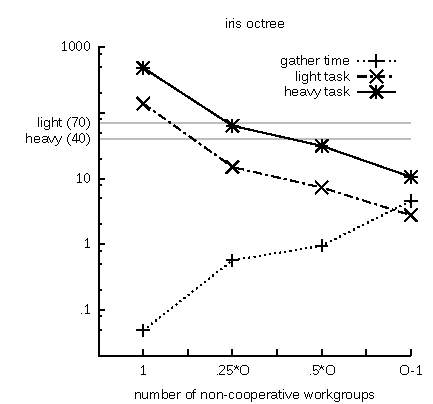
\includegraphics[width=.7\columnwidth]{iris_octree_NA.pdf} 
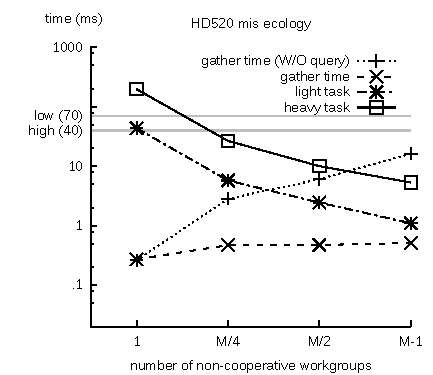
\includegraphics[width=.7\columnwidth]{hd520_mis_ecology.pdf}
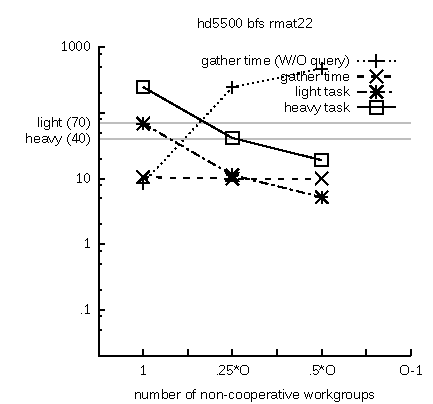
\includegraphics[width=.7\columnwidth]{hd5500_bfs_rmat22.pdf}
\caption{Example gather time and non-cooperative timing results}\label{fig:fine-grained-timing}
\end{figure*}


\section{Related Work}\label{sec:relatedwork}

\paragraph{Irregular algorithms and persistent kernels}

There has been a lot of work on accelerating blocking irregular
algorithms using GPUs, and on the \emph{persistent threads}
programming style for long-running kernels~\cite{owens-persistent,DBLP:conf/ipps/KaleemVPHP16,DBLP:conf/ipps/DavidsonBGO14,DBLP:conf/hipc/HarishN07,DBLP:journals/topc/MerrillGG15,DBLP:conf/egh/VineetHPN09,DBLP:conf/ppopp/NobariCKB12,DBLP:conf/hpcc/SolomonTT10a,DBLP:conf/popl/PrabhuRMH11,DBLP:conf/ppopp/Mendez-LojoBP12,DBLP:conf/oopsla/PaiP16,DBLP:conf/oopsla/SorensenDBGR16,dlb-web,TPO10,BNP12,Pannotia}.  These
approaches rely on the occupancy-bound execution model, and aim to
take ownership of the GPU by scheduling as many workgroups as the occupancy bound allows, relying on fair scheduling between these
workgroups.  This means the GPU is unavailable for other tasks, and
the method is not future-proof because (as discussed throughout the
paper) the occupancy-bound execution model is not guaranteed by GPU
programming models and is unlikely to be guaranteed in practice by
future GPU platforms.

As we have demonstrated for a representative set of irregular
algorithms, our cooperative kernels model allows blocking algorithms
to be upgraded to run under a fair scheduler in a manner that, with
appropriate care, facilitates responsive multitasking.

\paragraph{Preemptive multitasking on GPUs}

Hardware support for preemptive multitasking for \nvidia GPUs has been
proposed, enabling full preemption as well as \emph{SM-draining},
whereby workgroups occupying a symmetric multiprocessor (SM; a compute
unit using our terminology) are drained until the SM becomes free for
other tasks~\cite{DBLP:conf/isca/TanasicGCRNV14}.  A follow-up work adds the notion of SM \emph{flushing},
whereby a workgroup running on an SM can be cancelled and re-scheduled
from scratch if the workgroup has not yet committed any visible
side-effects to shared memory~\cite{DBLP:conf/asplos/ParkPM15}.  Both approaches have been evaluated
using simulators, over sets of regular GPU kernels.  State-of-the-art \nvidia GPUs targeting data centers (where multi-tasking is essential) do support
preemption, though it is not clear whether they guarantee fair scheduling~\cite{PascalWhitepaper}.

The advantages of these approaches are that they do not require manual
programmer effort, and the capability to fully preempt a workgroup
guards against a rogue long-running kernel making the GPU unavailable
for other tasks.  The drawbacks are that (a) because preemption is
enabled by default, \emph{every} kernel takes a potential performance
hit, and (b) the SM draining optimisation does not help in the case of
blocking algorithms (not considered in these works), since a blocked
workgroup cannot be drained.

Our solution does not impose a performance penalty on non-cooperative
kernels, which run in an unmodified manner, and careful placement of
our new language primitives can exploit the structure of a
cooperative kernel, enabling more efficient multitasking than
kernel-oblivious preemption.

There is scope for combining the approaches: if a
cooperative kernel is insufficiently cooperative, i.e.\ it does not
invoke $\offerkill$ enough, then hardware support for preemption could
be invoked to prevent the kernel from denying other tasks access to
the GPU indefinitely.

\paragraph{Optimizing GPU scheduling}
%
A number of works have considered how best to schedule dynamic
workloads on GPUs~\cite{DBLP:journals/tog/SteinbergerKKHKS12,DBLP:conf/ics/WuCLSV15,DBLP:conf/usenix/KatoLRI11,DBLP:journals/tog/SteinbergerKBKDS14,DBLP:journals/rts/ElliottA12,DBLP:conf/sosp/RossbachCSRW11}.  Among these, the Whippletree approach employs a persistent
megakernel to schedule multiple, dynamic tasks in a manner that aims
to best utilise GPU
resources~\cite{DBLP:journals/tog/SteinbergerKBKDS14}.  The TimeGraph
approach similarly aims to optimise scheduling of competing workloads,
in the context of OpenGL, using GPU-CPU synchronisation so that the
CPU can monitor and control the work that is scheduled on the
GPU~\cite{DBLP:conf/usenix/KatoLRI11}.  To best utilise the compute
units of a GPU for a particular kernel, SM-centric program
transformations have been proposed, which aim to direct work to
specific compute units, rather than to specific workgroups, based on
the observation that in practice multiple workgroups may share the
same compute unit, so that said workgrops might be in a good position
to exploit memory caches associated with that compute
unit~\cite{DBLP:conf/ics/WuCLSV15}.  None of these approaches tackle
the problem of \emph{fair} scheduling on GPUs that our work addresses, thus they do not aid in safe deployment of blocking irregular algorithms.

\paragraph{Dynamic parallelism} Recent versions of CUDA and OpenCL allow a kernel to spawn further kernels~\cite{cuda-75,opencl2Spec}.
This \emph{dynamic parallelism} can be exploited to implement a
GPU-based scheduler, by having an initial scheduler kernel repeatedly
spawn further kernels as required, according to some scheduling
policy~\cite{DBLP:conf/ppopp/Muyan-OzcelikO16}.  However, a kernel
that uses dynamic parallelism is still subject to the scheduling
limitations of current GPU programming models, and in particular the
problem that workgroups are not fairly scheduled.  Hence this feature
does not offer a solution to the problem of deploying blocking
algorithms on GPUs in a safe manner that we tackle with this work.

\paragraph{Cooperative multitasking}

Cooperative multitasking was offered in older operating systems
(e.g. Windows before the 95 edition) and is still used by some
operating systems, such as RISC
OS.\footnote{\url{http://www.riscos.info/index.php/Preemptive_multitasking}}
Many programming languages offer cooperative multitasking via
variations of coroutines, e.g. coroutine objects in
Python\footnote{\url{https://docs.python.org/3/reference/datamodel.html\#coroutine-objects}}
or Lua,\footnote{\url{https://www.lua.org/pil/9.1.html}} or Ruby's
\emph{fiber}.\footnote{\url{http://ruby-doc.org/core-2.1.1/Fiber.html}}

In the context of GPUs, cooperative multitasking has been used to
refer to the standard setup today, whereby the onus is on a GPU kernel
to complete execution within a reasonable time budget and return
control to the CPU application~\cite{adriaens2012case,CPE:CPE1722}.  In this setting, the programmer is responsible for ensuring cooperation between the host application and GPU kernel so that a kernel does not run for too long.
%
This is in contrast to our notion of cooperative kernels, which is designed specifically to support the needs of long-running kernels that one might wish to multitask with other workloads.


\section{Conclusions and Future Work}\label{sec:conclusion}

\ADComment{Do citation tidy-up.}

\ADComment{Next-generation GPUs and drivers for evaluation,
  implementation in a real driver, migration of work between multiple
  GPUs.}

\clearpage

\bibliographystyle{abbrvnat}
\bibliography{tyler}

\clearpage

\appendix

\section{Operational Semantics for Cooperative Kernels}\label{appendix:semantics}

\newcommand{\myss}{\mathit{ss}}
\newcommand{\Stmts}{\mathsf{Stmts}}
\newcommand{\threadstates}{\mathsf{ThreadStates}}
\newcommand{\sharedstates}{\mathsf{SharedStates}}
\newcommand{\sync}{\mathsf{sync}}

In \mysec\ref{sec:semantics} we presented the semantics of cooperative
kernels relatively informally, using English, to provide the intuition
behind our programmming model.  We now back this up with a more formal
presentation as an operational semantics for an abstract GPU
programming model.

\paragraph{States}

Let $L$ be a set of \emph{local states} that abstractly captures the
private memory associated with a thread executing a GPU kernel.  Let
$\Stmts$ denote the set of all possible statements that a
thread can execute.  We do not detail the structure of these
statements, except that we assume sequential composition of statements
is provided by the $\code{;}$ separator, and that the $\offerkill$,
$\offerfork$, $\globalbarrier$ and $\resizingglobalbarrier$ primitives
from our cooperative kernels programming model are valid statements.

A \emph{thread state} is then a pair $(l, \myss)$, where $l \in L$ and
$\myss \in \Stmts$.  The $l$ component captures the valuation of all the
thread's private memory, and the $\myss$ component captures the
remaining statements to be executed by the thread.  Let $\threadstates$ denote the set of all thread states.

Assuming that $d > 0$ threads per workgroup were requested on kernel launch, a \emph{workgroup state}
is a $d$-tuple $((l_0, \myss_0), \dots, (l_{d-1}, \myss_{d-1}))$, where each $(l_i, \myss_i)$ is the thread state for the $i$th thread in the workgroup $(0\leq i < d$).

Assuming that $N > 0$ was specified as the maximum number of
workgroups that should execute the cooperative kernel, a \emph{kernel
  state} is then a pair
%
\[
(\sigma, (w_0, \dots, w_{M-1}, \underbrace{\bot, \dots,
\bot}_{N-M}))\]
%
where: $\sigma$ represents the shared state of the kernel; $M \leq N$
is the number of \emph{active} workgroups; $w_i$ is the workgroup
state for active workgroup $i$ ($0 \leq i < M$); and $N-M$ occurrences
of $\bot$ indicate \emph{absent} workgroups.  Let $\sharedstates$
denote the set of all possible shared states.  We regard
workgroup-local storage as being part of the shared state of a kernel.

\paragraph{Thread-level transitions}

We leave the semantics for thread-level transitions abstract, assuming
a binary relation $\rightarrow_{tau}$ on $\sharedstates{} \times
\threadstates{}$.  If $(\sigma, (l, \myss)) \rightarrow_{\tau}
(\sigma', (l', \myss'))$, this indicates that if a thread is in local
state $(l, \myss)$, the thread can transition to local state $(l',
\myss')$, changing the shared state from $\sigma$ to $\sigma'$ in the
process.

All we require is that $(\sigma, (l, \myss)) \rightarrow_{\tau}
(\sigma', (l', \myss'))$ if $\myss$ has the form $\mathsf{special}();
\mathit{tt}$, where $\mathsf{special}$ is one of $\offerkill$,
$\offerfork$, $\globalbarrier$ or $\resizingglobalbarrier$.  This is
because we shall specifically define the meaning of the new primitives
introduced by our programming model.

\paragraph{Memory synchronisation}

GPUs are known to have relaxed memory models~\cite{ABDGKPSW-2015}.  To abstractly
account for this, we assume that the shared state component $\sigma$
is not simplyl a mapping from locations to values, but instead
captures all the intricacies of GPU memory that can lead to this
relaxed behaviour.  We also assume a function $\sync$ which, given a
kernel state $\kappa$, returns a set of kernel states.  The idea is
that each $\kappa' \in \sync(\kappa)$ is a possible kernel state that
can be reached from $\kappa$ by stalling until all stores to memory
and loads from memory to thread-local storage have completed.  All we
require is that $\sync$ does not modify the number of active
workgroups nor the component of a thread state that determines which
statements remain to be executed.

\begin{figure*}
\begin{center}

\[
\inferrule{
w_i(j) = (l, \myss)
\\
(\sigma, (l, \myss)) \rightarrow_{\tau} (\sigma', (l', \myss'))
\\
w_i' = w_i[j \mapsto (l', \myss')]
}
{
(\sigma, (\dots, w_i, \dots)) \rightarrow (\sigma', (\dots, w_i', \dots))
}
(\textsc{Thread-Step})
\]

\medskip

\[
\inferrule{
\forall j \;.\; w_i(j) = (l_j, \offerkill();\myss)
\\
w_i' = ((l_0, \myss), \dots, (l_{d-1}, \myss))
}
{
(\sigma, (\dots, w_i, \dots)) \rightarrow (\sigma, (\dots, w_i', \dots))
}
(\textsc{Kill-No-Op})
\]

\medskip

\[
\inferrule{
\forall j \;.\; w_{M-1}(j) = (l_j, \offerkill();\myss)
\\
M > 0
}
{
(\sigma, (\dots, w_{M-2}, w_{M-1}, \bot, \dots, \bot)) \rightarrow (\sigma, (\dots, w_{M-2}, \bot, \bot, \dots, \bot))
}
(\textsc{Kill})
\]

\medskip

\[
\inferrule{
\forall j \;.\; w_i(j) = (l_j, \offerfork();\myss)
\\
w_i' = ((l_{0}, \myss), \dots, (l_{d-1}, \myss))
\\
k \in [0, N - M]
\\
\forall a \in [0, k - 1] \;.\; w_{M+a} = ((l_{0}, \myss), \dots, (l_{0}, \myss))
}
{
(\sigma, (\dots, w_i, \dots, w_{M-1}, \bot, \dots, \bot)) \rightarrow (\sigma, (\dots, w_i', \dots, w_{M-1}, w_{M}, \dots, w_{M+k-1}, \bot, \dots, \bot))
}
(\textsc{Fork})
\]

\medskip

\[
\inferrule{
\forall i \;.\;\forall j\;.\;w_i(j) = (l_{i,j}, \globalbarrier();\myss)
\\
\forall i \;.\;\forall j\;.\;w_i'(j) = (l_{i,j}, \myss)
\\\\
\kappa \in \sync((\sigma , (w_{0}', \dots, w_{M-1}', \bot, \dots, \bot))
}
{
(\sigma, (w_{0}, \dots, w_{M-1}, \bot, \dots, \bot)) \rightarrow \kappa
}
(\textsc{Barrier})
\]

\medskip

\[
\inferrule{
\forall i \;.\;\forall j\;.\;w_i(j) = (l_{i,j}, \resizingglobalbarrier();\myss)
\\
\forall j\;.\;w_{0}'(j) = (l_{1,j}, \globalbarrier(); \offerfork(); \globalbarrier(); \globalbarrier();\myss)
\\
\forall i \neq 1 \;.\;\forall j\;.\;w_i'(j) = (l_{i,j}, \globalbarrier(); \globalbarrier(); \offerkill(); \globalbarrier();\myss)
}
{
(\sigma, (w_{0}, \dots, w_{M-1}, \bot, \dots, \bot)) \rightarrow (\sigma, (w_{0}', \dots, w_{M-1}', \bot, \dots, \bot))
}
(\textsc{Resizing-Barrier})
\]

\end{center}

\caption{Abstract operational semantics for our cooperative kernels language extensions}\label{fig:semanticrules}

\end{figure*}

\paragraph{Operational semantics rules}

\myfiglong\ref{fig:semanticrules} presents the rules of our
operational semantics, defining a relation $\rightarrow$ on kernel
states.

Rule $\textsc{Thread-Step}$ defines the semantics for thread making a
single execution step, delegating to the abstract $\rightarrow_{\tau}$
relation to determine how the thread's local state and the shared
state component change.  For simplicity, this rule ignores the
semantics of intra-workgroup barriers, which are not our focus here.

Rule $\textsc{Kill-No-Op}$ reflects the fact that when a workgroup
reaches $\offerkill$, this can always be treated as a no-op.  Whether
a scheduler implementation accepts $\offerkill$ calls or not depends
on competing workloads and how the scheduler has been designed to meet
the non-functinoal requirements discussed in
\mysec\ref{sec:nonfunctional}, but in general the programmer should
always be prepared for the possiblity that a workgroup survives after
calling $\offerkill$.

The case where a workgroup's offer to be killed is accepted by the
scheduler is captured by rule $\textsc{Kill}$.  Because we have
adopted a semantics where workgroup 0 is never killed and where only
the workgroup with the highest id can be killed, the rule only fires
if $M > 0$ and workgroup $M-1$ has reached $\offerkill$.  The rule has
the effect of replacing the workgroup state for $w_{M-1}$
with $\bot$.

Recall that $\offerkill$ is a workgroup-level function: the same
syntactic $\offerfork$ call must be reached by all threads in a
workgroup.  This is captured in our rules by requiring in both
$\textsc{Kill-No-Op}$ and $\textsc{Kill}$ that every thread is ready
to execute $\offerkill$ followed by an identical statement $\myss$.
Neither rule applies until all threads in a workgroup reach
$\offerfork$, and the workgroup gets stuck if multiple threads in a
workgroiup reach $\offerfork$ with different subsequent statements.

The $\textsc{Fork}$ rule similarly requires all threads in a workgroup
to reach $\offerfork$ with identical following statements.  A
nondeterministic number of new workgroups, $k$, is selected to be
forked, where $k \in [0, N-M]$.  Importantly, $k=0$ is always a
legitimate choice, in which case $\offerfork$ has no effect on the
number of workgroups that are executing.  In the case where $k > 0$,
$k$ new workgroup states are created, where each workgroup inherits
the local state of thread 0 in $w_i$, the workgroup executing the fork
call.  After $\offerfork$, all threads in all workgroups, including
the new threads, proceed to execute the sequence of statements $\myss$
that followed $\offerfork$.

A simplification here is that we do not model transmission of
particular annotated variables from thread 0 of the forking workgroup,
instead specifying that the entire local state of the workgroup is
transmitted.  Extending the semantics to transmit only annotated
variables would be straightforward but verbose, requiring the local
memory component of a thread state to be split into two: the part of
the local state to be transmitted (modelling $\transmit$-annotated
variables), and the rest of the local state.

The $\textsc{Barrier}$ rule requires that \emph{every} thread
executing the kernel reaches $\globalbarrier()$ an identical following
statement.  This reflects that fact that $\globalbarrier()$ is a
kernel-level function.  Each thread then skips over the
$\globalbarrier()$ call, and the $\sync$ function is applied to yield
a set of kernel states that can arise due to memory synchronization
taking place.  An arbitary member of this set is selected as the next
kernel state.

Despite its apparent complexity, the $\textsc{Resizing-Barrier}$ rule simply implements the rewriting of $\resizingglobalbarrier$ in terms of $\globalbarrier$, $\offerkill$ and $\offerfork$ discussed in \mysec\ref{ }.


\section{Alternative Semantic Choices}\label{appendix:semanticalternatives}

The semantics of cooperative kernels has been guided by the practical
applications we have studied (described in
\mysec\ref{sec:portingalgorithms}).  We now discuss several cases
where we might have taken different and also reasonable semantic
decisions.

\paragraph{Killing order}

We opted for a semantics whereby only the active workgroup with the
highest id can be killed.  This has an appealing property: it means
that the ids of active workgroups are contiguous, which is important
for processing of contiguous data.  The cooperative graph traversal
algorithm of \myfig\ref{fig:cgraphsearch} illustrates this: the
algorithm is prepared for $\getglobalsize()$ to change after each
resizing barrier call, but depends on the fact that $\getglobalid()$
returns a contiguous range of thread ids.

A disadvantage of this decision is that it may provide sub-optimal
responsiveness from the point of view of the scheduler.  Suppose the
scheduler requires an additional compute unit, but the active thread
with the larget id is processing some computationally intensive work
and will take a while to reach $\offerkill$.  Our semantics means that
the scheuduler cannot take advantage of the fact that another active
workgroup may invoke $\offerkill$ sooner.

Cooperative kernels that do not require contiguous thread ids might me
more suited to a semantics in which workgroups can be killed in any
order, but where workgroup ids (and thus thread global ids) are not
guaranteed to be contiguous.

\paragraph{Keeping one workgroup alive}

Our semantics dictate that the workgroup with id 0 will not be killed
if it invokes $\offerkill$.  This avoids the possibility of the
cooperative kernel terminating early due to the programmer
inadvertantly allowing all workgroups to be killed, and the decision
to keep workgroup 0 alive fits well with our choice to kill workgroups
in descending order of id.

However, there might be a use case for a cooperative kernel reaching a
point where it would be acceptable for the kernel to exit, although
desirable for some remaining computation to be performed if competing
workloads allow it.  In this case, a semantics where all workgroups can be killed via $\offerkill$ would be appropriate, and the programmer would need to guard each $\offerkill$ with an id check in cases where killing all workgroups would be unacceptable.  For example:
%
\lstset{basicstyle=\tt,numbers=none}
\begin{lstlisting}
  if($\getgroupid{0}$ != 0) $\offerkill$();
\end{lstlisting}
\lstset{basicstyle=\scriptsize\tt,numbers=left}
%
would ensure that at least workgroup 0 is kept alive.

\paragraph{Transmission of partial state from a single thread}

Recall from the semantics of $\offerfork$ that newly forked workgroups
inherit the variable valuation associated with thread 0 of the forking
workgroup, but only for $\transmit$-annotated variables.  Alternative
choices here would be to have forked workgroups inherit values for
\emph{all} variables from the forking workgroup, and to have thread
$i$ in the forking workgroup provide the valuation for thread $i$ in
each spawned workgroup, rather than having thread 0 transmit the
valuation to all new threads.

We opted for transmitting only selected varibles based on the
observation that many of a thread's private variables are dead at the
point of issuing $\offerfork$ or $\resizingglobalbarrier$, thus it
would be wasteful to transmit them.  A live variable analysis could
instead be employed to over-approximate the variables that might be
accessed by newly arriving workgroups, so that these are automatically
transmitted.

In all cases, we found that a variable that needed to be transmitted
had the property of being uniform across the workgroup.  That is,
despite each thread having its own copy of the variable, each thread
is in agreement on the variable's value.  As an example, the
$\keyword{level}$, $\keyword{in\_nodes}$ and $\keyword{out\_nodes}$
variables used in \myfig\ref{fig:cgraphsearch} are all stored in thread-private
memory, but all threads in a workgroup agree on the values of these
variables at each $\resizingglobalbarrier$ call.  As a result,
transmitting the thread 0's valuation of the annotated variables is
equivalent to (and more efficient than) transmitting values on a
thread-by-thread basis.  We have not yet encountered a real-world
example where our current semantics would not suffice.


\section{Full Set of Graphs for Responsiveness Experiments}

\ADComment{TODO: we need this.  Probably not the right title.}


\end{document}
